\documentclass[twoside]{book}

% Packages required by doxygen
\usepackage{calc}
\usepackage{doxygen}
\usepackage{graphicx}
\usepackage[utf8]{inputenc}
\usepackage{makeidx}
\usepackage{multicol}
\usepackage{multirow}
\usepackage{textcomp}
\usepackage[table]{xcolor}

% Font selection
\usepackage[T1]{fontenc}
\usepackage{mathptmx}
\usepackage[scaled=.90]{helvet}
\usepackage{courier}
\usepackage{amssymb}
\usepackage{sectsty}
\renewcommand{\familydefault}{\sfdefault}
\allsectionsfont{%
  \fontseries{bc}\selectfont%
  \color{darkgray}%
}
\renewcommand{\DoxyLabelFont}{%
  \fontseries{bc}\selectfont%
  \color{darkgray}%
}

% Page & text layout
\usepackage{geometry}
\geometry{%
  a4paper,%
  top=2.5cm,%
  bottom=2.5cm,%
  left=2.5cm,%
  right=2.5cm%
}
\tolerance=750
\hfuzz=15pt
\hbadness=750
\setlength{\emergencystretch}{15pt}
\setlength{\parindent}{0cm}
\setlength{\parskip}{0.2cm}
\makeatletter
\renewcommand{\paragraph}{%
  \@startsection{paragraph}{4}{0ex}{-1.0ex}{1.0ex}{%
    \normalfont\normalsize\bfseries\SS@parafont%
  }%
}
\renewcommand{\subparagraph}{%
  \@startsection{subparagraph}{5}{0ex}{-1.0ex}{1.0ex}{%
    \normalfont\normalsize\bfseries\SS@subparafont%
  }%
}
\makeatother

% Headers & footers
\usepackage{fancyhdr}
\pagestyle{fancyplain}
\fancyhead[LE]{\fancyplain{}{\bfseries\thepage}}
\fancyhead[CE]{\fancyplain{}{}}
\fancyhead[RE]{\fancyplain{}{\bfseries\leftmark}}
\fancyhead[LO]{\fancyplain{}{\bfseries\rightmark}}
\fancyhead[CO]{\fancyplain{}{}}
\fancyhead[RO]{\fancyplain{}{\bfseries\thepage}}
\fancyfoot[LE]{\fancyplain{}{}}
\fancyfoot[CE]{\fancyplain{}{}}
\fancyfoot[RE]{\fancyplain{}{\bfseries\scriptsize Generated on Tue Mar 25 2014 01\-:12\-:19 for S\-K\-J by Doxygen }}
\fancyfoot[LO]{\fancyplain{}{\bfseries\scriptsize Generated on Tue Mar 25 2014 01\-:12\-:19 for S\-K\-J by Doxygen }}
\fancyfoot[CO]{\fancyplain{}{}}
\fancyfoot[RO]{\fancyplain{}{}}
\renewcommand{\footrulewidth}{0.4pt}
\renewcommand{\chaptermark}[1]{%
  \markboth{#1}{}%
}
\renewcommand{\sectionmark}[1]{%
  \markright{\thesection\ #1}%
}

% Indices & bibliography
\usepackage{natbib}
\usepackage[titles]{tocloft}
\setcounter{tocdepth}{3}
\setcounter{secnumdepth}{5}
\makeindex

% Hyperlinks (required, but should be loaded last)
\usepackage{ifpdf}
\ifpdf
  \usepackage[pdftex,pagebackref=true]{hyperref}
\else
  \usepackage[ps2pdf,pagebackref=true]{hyperref}
\fi
\hypersetup{%
  colorlinks=true,%
  linkcolor=blue,%
  citecolor=blue,%
  unicode%
}

% Custom commands
\newcommand{\clearemptydoublepage}{%
  \newpage{\pagestyle{empty}\cleardoublepage}%
}


%===== C O N T E N T S =====

\begin{document}

% Titlepage & ToC
\hypersetup{pageanchor=false}
\pagenumbering{roman}
\begin{titlepage}
\vspace*{7cm}
\begin{center}%
{\Large S\-K\-J }\\
\vspace*{1cm}
{\large Generated by Doxygen 1.8.5}\\
\vspace*{0.5cm}
{\small Tue Mar 25 2014 01:12:19}\\
\end{center}
\end{titlepage}
\clearemptydoublepage
\tableofcontents
\clearemptydoublepage
\pagenumbering{arabic}
\hypersetup{pageanchor=true}

%--- Begin generated contents ---
\chapter{Main Page}
\label{index}\hypertarget{index}{}{\ttfamily ioskj} is a simulation model of the Indian Ocean skipjack tuna fishery for management strategy evaluation.

\subsection*{Status}

{\ttfamily ioskj} is still under active development. It requires several third party C++ libraries and a modern C++ compiler which supports the C++11 standard. At this stage we do not recommend trying to compile it yourself. As the model matures we intend to make it available as precompiled executables for Windows and Linux and/or a package for R.

\subsection*{Documentation}

Documentation is at \href{http://trophia.github.io/ioskj/}{\tt http\-://trophia.\-github.\-io/ioskj/}

\subsection*{Organisation}

\subsubsection*{C++ files}

The main C++ files are\-:


\begin{DoxyItemize}
\item {\ttfamily \hyperlink{dimensions_8hpp_source}{dimensions.\-hpp}} -\/ defines the dimensions used in various model arrays e.\-g. {\ttfamily Region}, {\ttfamily Age}, {\ttfamily Method}
\item {\ttfamily \hyperlink{fish_8hpp_source}{fish.\-hpp}} -\/ contains the {\ttfamily Fish} class representing the fish population dynamic
\item {\ttfamily \hyperlink{fishing_8hpp_source}{fishing.\-hpp}} -\/ contains the {\ttfamily Fishing} class representing fishing activity
\item {\ttfamily \hyperlink{data_8hpp_source}{data.\-hpp}} -\/ reads in and holds data for use in driving and conditioning the model
\item {\ttfamily \hyperlink{model_8hpp_source}{model.\-hpp}} -\/ contains the {\ttfamily Model} class which puts {\ttfamily Fish}, {\ttfamily Fishing} and the various data classes together
\item {\ttfamily main.\-cpp} -\/ the primary C++ file for compiling a {\ttfamily Model} executable
\end{DoxyItemize}

\subsubsection*{{\ttfamily data} folder}

The {\ttfamily data} folder includes R and Python scripts for processing source data. See the documentation in those files for more details. The resulting, processed data is outputted to the folder {\ttfamily data\textbackslash{}processed-\/data}.

\subsubsection*{{\ttfamily docs} folder}

The {\ttfamily docs} folder includes hand written documentation and a Doxygen project for automatically generating documentation from C++ source code/ 
\chapter{Test List}
\label{test}
\hypertarget{test}{}

\begin{DoxyRefList}
\item[\label{test__test000001}%
\hypertarget{test__test000001}{}%
Class \hyperlink{classIOSKJ_1_1Model}{I\-O\-S\-K\-J\-:\-:Model} ]equilibrium\-\_\-stable

equilibrium\-\_\-uniform

recruiment\-\_\-variation

exploitation\-\_\-specified
\end{DoxyRefList}
\chapter{Hierarchical Index}
\section{Class Hierarchy}
This inheritance list is sorted roughly, but not completely, alphabetically\-:\begin{DoxyCompactList}
\item Data\-Group\begin{DoxyCompactList}
\item \contentsline{section}{I\-O\-S\-K\-J\-:\-:Data}{\pageref{classIOSKJ_1_1Data}}{}
\end{DoxyCompactList}
\item Dimension\begin{DoxyCompactList}
\item \contentsline{section}{I\-O\-S\-K\-J\-:\-:Data\-Year}{\pageref{classIOSKJ_1_1DataYear}}{}
\item \contentsline{section}{I\-O\-S\-K\-J\-:\-:Year}{\pageref{classIOSKJ_1_1Year}}{}
\end{DoxyCompactList}
\item \contentsline{section}{I\-O\-S\-K\-J\-:\-:Model}{\pageref{classIOSKJ_1_1Model}}{}
\item \contentsline{section}{model\-Fixture}{\pageref{structmodelFixture}}{}
\item Parameter\-Group\begin{DoxyCompactList}
\item \contentsline{section}{I\-O\-S\-K\-J\-:\-:Parameters}{\pageref{classIOSKJ_1_1Parameters}}{}
\end{DoxyCompactList}
\item \contentsline{section}{I\-O\-S\-K\-J\-:\-:Tracker}{\pageref{structIOSKJ_1_1Tracker}}{}
\end{DoxyCompactList}

\chapter{Class Index}
\section{Class List}
Here are the classes, structs, unions and interfaces with brief descriptions\-:\begin{DoxyCompactList}
\item\contentsline{section}{\hyperlink{classIOSKJ_1_1Fish}{I\-O\-S\-K\-J\-::\-Fish} }{\pageref{classIOSKJ_1_1Fish}}{}
\item\contentsline{section}{\hyperlink{classIOSKJ_1_1Fishing}{I\-O\-S\-K\-J\-::\-Fishing} }{\pageref{classIOSKJ_1_1Fishing}}{}
\item\contentsline{section}{\hyperlink{structGenerator}{Generator} }{\pageref{structGenerator}}{}
\item\contentsline{section}{\hyperlink{classIOSKJ_1_1Data_1_1MaldivePlCpue}{I\-O\-S\-K\-J\-::\-Data\-::\-Maldive\-Pl\-Cpue} }{\pageref{classIOSKJ_1_1Data_1_1MaldivePlCpue}}{}
\item\contentsline{section}{\hyperlink{classIOSKJ_1_1Model}{I\-O\-S\-K\-J\-::\-Model} }{\pageref{classIOSKJ_1_1Model}}{}
\item\contentsline{section}{\hyperlink{classIOSKJ_1_1Data_1_1NominalCatch}{I\-O\-S\-K\-J\-::\-Data\-::\-Nominal\-Catch} }{\pageref{classIOSKJ_1_1Data_1_1NominalCatch}}{}
\item\contentsline{section}{\hyperlink{classIOSKJ_1_1Data_1_1SizeFrequency}{I\-O\-S\-K\-J\-::\-Data\-::\-Size\-Frequency} }{\pageref{classIOSKJ_1_1Data_1_1SizeFrequency}}{}
\item\contentsline{section}{\hyperlink{classIOSKJ_1_1Data_1_1WestPsCpue}{I\-O\-S\-K\-J\-::\-Data\-::\-West\-Ps\-Cpue} }{\pageref{classIOSKJ_1_1Data_1_1WestPsCpue}}{}
\item\contentsline{section}{\hyperlink{classIOSKJ_1_1Data_1_1ZEstimate}{I\-O\-S\-K\-J\-::\-Data\-::\-Z\-Estimate} }{\pageref{classIOSKJ_1_1Data_1_1ZEstimate}}{}
\end{DoxyCompactList}

\chapter{Class Documentation}
\hypertarget{classIOSKJ_1_1Data}{\section{I\-O\-S\-K\-J\-:\-:Data Class Reference}
\label{classIOSKJ_1_1Data}\index{I\-O\-S\-K\-J\-::\-Data@{I\-O\-S\-K\-J\-::\-Data}}
}


{\ttfamily \#include $<$data.\-hpp$>$}

Inheritance diagram for I\-O\-S\-K\-J\-:\-:Data\-:\begin{figure}[H]
\begin{center}
\leavevmode
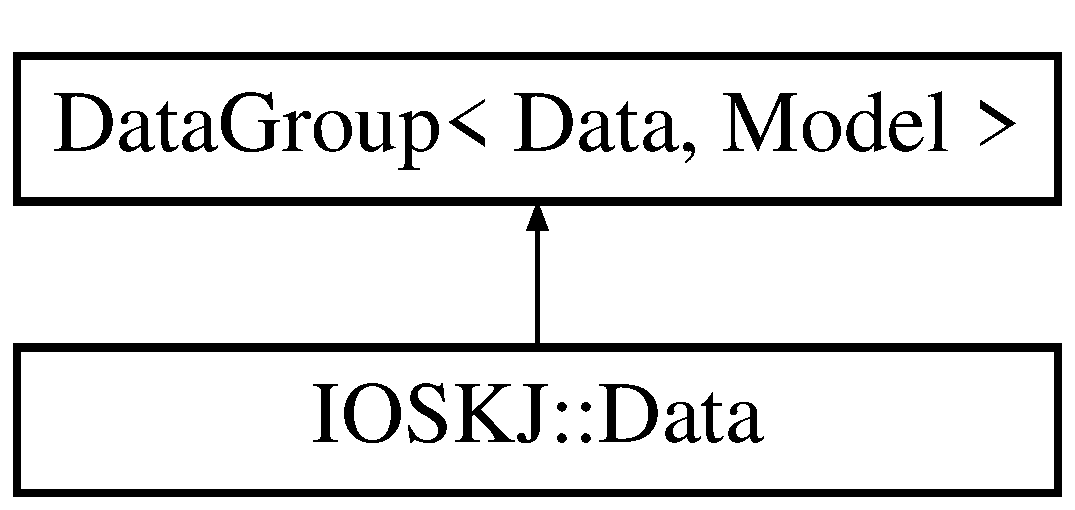
\includegraphics[height=2.000000cm]{classIOSKJ_1_1Data}
\end{center}
\end{figure}
\subsection*{Public Member Functions}
\begin{DoxyCompactItemize}
\item 
void \hyperlink{classIOSKJ_1_1Data_a36ad666102014528bb511c680cc0db27}{get} (const \hyperlink{classIOSKJ_1_1Model}{Model} \&model, uint time)
\item 
double \hyperlink{classIOSKJ_1_1Data_af00399104402b9bbd8d01292f8b28e17}{likelihood} (void)
\item 
void \hyperlink{classIOSKJ_1_1Data_afbfbcac4c122782aace3315096e8b402}{read} (void)
\item 
void \hyperlink{classIOSKJ_1_1Data_ab5f18a8f4dfc4b720599f066c717ecae}{write} (void)
\end{DoxyCompactItemize}
\subsection*{Public Attributes}
\begin{DoxyCompactItemize}
\item 
\hypertarget{classIOSKJ_1_1Data_aa3b2e824ab3da78d2cdd690f1a4f16d8}{Fits$<$ Lognormal, \hyperlink{classIOSKJ_1_1DataYear}{Data\-Year}, \\*
Quarter $>$ {\bfseries m\-\_\-pl\-\_\-cpue} = 0.\-2}\label{classIOSKJ_1_1Data_aa3b2e824ab3da78d2cdd690f1a4f16d8}

\item 
\hypertarget{classIOSKJ_1_1Data_af9efd9cde37d159fba07a24a0658d129}{Fits$<$ Lognormal, \hyperlink{classIOSKJ_1_1DataYear}{Data\-Year} $>$ {\bfseries w\-\_\-ps\-\_\-cpue} = 0.\-3}\label{classIOSKJ_1_1Data_af9efd9cde37d159fba07a24a0658d129}

\item 
\hypertarget{classIOSKJ_1_1Data_ac4664d2235f7278fd70684ee866c0c7d}{Fits$<$ Normal, \hyperlink{classIOSKJ_1_1DataYear}{Data\-Year}, \\*
Quarter, Region, Method, Size $>$ {\bfseries size\-\_\-freqs} = 0.\-01}\label{classIOSKJ_1_1Data_ac4664d2235f7278fd70684ee866c0c7d}

\item 
\hypertarget{classIOSKJ_1_1Data_ab5a1f2a231f8569312e7d8446709fad7}{Fits$<$ Normal, \hyperlink{classIOSKJ_1_1DataYear}{Data\-Year}, \\*
Quarter, Z\-Size $>$ {\bfseries z\-\_\-ests} = 0.\-05}\label{classIOSKJ_1_1Data_ab5a1f2a231f8569312e7d8446709fad7}

\end{DoxyCompactItemize}


\subsection{Detailed Description}
Class for defining data against which the model is conditioned See the {\ttfamily \hyperlink{classIOSKJ_1_1Data_a36ad666102014528bb511c680cc0db27}{get()}} method which \char`\"{}gets\char`\"{} model variables corresponding to data points at specific times. 

\subsection{Member Function Documentation}
\hypertarget{classIOSKJ_1_1Data_a36ad666102014528bb511c680cc0db27}{\index{I\-O\-S\-K\-J\-::\-Data@{I\-O\-S\-K\-J\-::\-Data}!get@{get}}
\index{get@{get}!IOSKJ::Data@{I\-O\-S\-K\-J\-::\-Data}}
\subsubsection[{get}]{\setlength{\rightskip}{0pt plus 5cm}void I\-O\-S\-K\-J\-::\-Data\-::get (
\begin{DoxyParamCaption}
\item[{const {\bf Model} \&}]{model, }
\item[{uint}]{time}
\end{DoxyParamCaption}
)\hspace{0.3cm}{\ttfamily [inline]}}}\label{classIOSKJ_1_1Data_a36ad666102014528bb511c680cc0db27}
Get model variables corresponding to data at a particular time

For each data set, predictions are generated outside of the range of observed data. This is for diagnosis and future proofing (when more observed data become available and are added to data files the model will already be set up to fit that it). There will be a small computational cost to this. \hypertarget{classIOSKJ_1_1Data_af00399104402b9bbd8d01292f8b28e17}{\index{I\-O\-S\-K\-J\-::\-Data@{I\-O\-S\-K\-J\-::\-Data}!likelihood@{likelihood}}
\index{likelihood@{likelihood}!IOSKJ::Data@{I\-O\-S\-K\-J\-::\-Data}}
\subsubsection[{likelihood}]{\setlength{\rightskip}{0pt plus 5cm}double I\-O\-S\-K\-J\-::\-Data\-::likelihood (
\begin{DoxyParamCaption}
\item[{void}]{}
\end{DoxyParamCaption}
)\hspace{0.3cm}{\ttfamily [inline]}}}\label{classIOSKJ_1_1Data_af00399104402b9bbd8d01292f8b28e17}
Calculate the log-\/likelihood of the fits to the data \hypertarget{classIOSKJ_1_1Data_afbfbcac4c122782aace3315096e8b402}{\index{I\-O\-S\-K\-J\-::\-Data@{I\-O\-S\-K\-J\-::\-Data}!read@{read}}
\index{read@{read}!IOSKJ::Data@{I\-O\-S\-K\-J\-::\-Data}}
\subsubsection[{read}]{\setlength{\rightskip}{0pt plus 5cm}void I\-O\-S\-K\-J\-::\-Data\-::read (
\begin{DoxyParamCaption}
\item[{void}]{}
\end{DoxyParamCaption}
)\hspace{0.3cm}{\ttfamily [inline]}}}\label{classIOSKJ_1_1Data_afbfbcac4c122782aace3315096e8b402}
Read in observed data \hypertarget{classIOSKJ_1_1Data_ab5f18a8f4dfc4b720599f066c717ecae}{\index{I\-O\-S\-K\-J\-::\-Data@{I\-O\-S\-K\-J\-::\-Data}!write@{write}}
\index{write@{write}!IOSKJ::Data@{I\-O\-S\-K\-J\-::\-Data}}
\subsubsection[{write}]{\setlength{\rightskip}{0pt plus 5cm}void I\-O\-S\-K\-J\-::\-Data\-::write (
\begin{DoxyParamCaption}
\item[{void}]{}
\end{DoxyParamCaption}
)\hspace{0.3cm}{\ttfamily [inline]}}}\label{classIOSKJ_1_1Data_ab5f18a8f4dfc4b720599f066c717ecae}
Write out fits 

The documentation for this class was generated from the following file\-:\begin{DoxyCompactItemize}
\item 
data.\-hpp\end{DoxyCompactItemize}

\hypertarget{classIOSKJ_1_1DataYear}{\section{I\-O\-S\-K\-J\-:\-:Data\-Year Class Reference}
\label{classIOSKJ_1_1DataYear}\index{I\-O\-S\-K\-J\-::\-Data\-Year@{I\-O\-S\-K\-J\-::\-Data\-Year}}
}
Inheritance diagram for I\-O\-S\-K\-J\-:\-:Data\-Year\-:\begin{figure}[H]
\begin{center}
\leavevmode
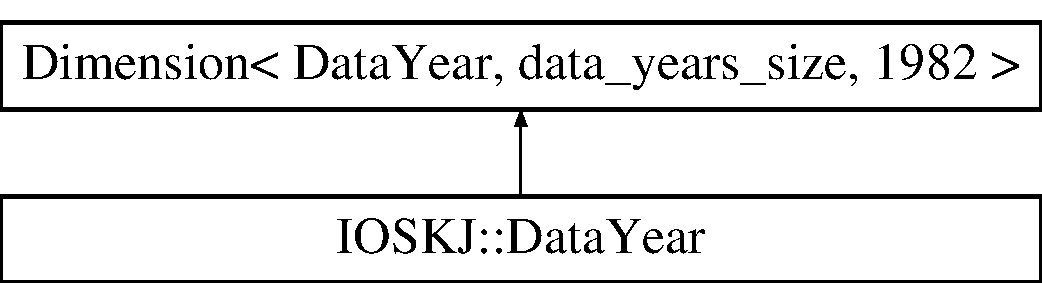
\includegraphics[height=2.000000cm]{classIOSKJ_1_1DataYear}
\end{center}
\end{figure}
\subsection*{Static Public Member Functions}
\begin{DoxyCompactItemize}
\item 
\hypertarget{classIOSKJ_1_1DataYear_ad010dabb07a1be03f32d062deb360963}{static const char $\ast$ {\bfseries name} (void)}\label{classIOSKJ_1_1DataYear_ad010dabb07a1be03f32d062deb360963}

\end{DoxyCompactItemize}


The documentation for this class was generated from the following file\-:\begin{DoxyCompactItemize}
\item 
dimensions.\-hpp\end{DoxyCompactItemize}

\hypertarget{classIOSKJ_1_1Model}{\section{I\-O\-S\-K\-J\-:\-:Model Class Reference}
\label{classIOSKJ_1_1Model}\index{I\-O\-S\-K\-J\-::\-Model@{I\-O\-S\-K\-J\-::\-Model}}
}
\subsection*{Public Member Functions}
\begin{DoxyCompactItemize}
\item 
\hypertarget{classIOSKJ_1_1Model_ae261a53c42f71d17182c1b129698126d}{void {\bfseries track\-\_\-begin} (void)}\label{classIOSKJ_1_1Model_ae261a53c42f71d17182c1b129698126d}

\item 
\hypertarget{classIOSKJ_1_1Model_af18a3687dd2685745174b91e0aae56ce}{void {\bfseries track} (void)}\label{classIOSKJ_1_1Model_af18a3687dd2685745174b91e0aae56ce}

\item 
\hypertarget{classIOSKJ_1_1Model_a03e6aeb637c83c34774ac66c18bac74d}{void {\bfseries track\-\_\-end} (void)}\label{classIOSKJ_1_1Model_a03e6aeb637c83c34774ac66c18bac74d}

\item 
\hypertarget{classIOSKJ_1_1Model_a6f42bfc7352faa7bba7e00d04fc166b0}{void {\bfseries startup} (void)}\label{classIOSKJ_1_1Model_a6f42bfc7352faa7bba7e00d04fc166b0}

\item 
\hypertarget{classIOSKJ_1_1Model_abf9ebdb10aee501808836438cb542fab}{void {\bfseries simulate} (void)}\label{classIOSKJ_1_1Model_abf9ebdb10aee501808836438cb542fab}

\item 
\hypertarget{classIOSKJ_1_1Model_a343216d7c9019f15f01f205423001005}{void {\bfseries shutdown} (void)}\label{classIOSKJ_1_1Model_a343216d7c9019f15f01f205423001005}

\end{DoxyCompactItemize}
\subsection*{Public Attributes}
\begin{DoxyCompactItemize}
\item 
\hypertarget{classIOSKJ_1_1Model_aa8bf5f43996857e428bb0745943363a4}{\hyperlink{classIOSKJ_1_1Fish}{Fish} {\bfseries fish}}\label{classIOSKJ_1_1Model_aa8bf5f43996857e428bb0745943363a4}

\item 
\hypertarget{classIOSKJ_1_1Model_a416c537ca8c64648516e928fcea72ef2}{\hyperlink{classIOSKJ_1_1Fishing}{Fishing} {\bfseries fishing}}\label{classIOSKJ_1_1Model_a416c537ca8c64648516e928fcea72ef2}

\end{DoxyCompactItemize}


The documentation for this class was generated from the following file\-:\begin{DoxyCompactItemize}
\item 
/home/nbentley/\-Trophia/\-Code/ioskj/model.\-hpp\end{DoxyCompactItemize}

\hypertarget{structmodelFixture}{\section{model\-Fixture Struct Reference}
\label{structmodelFixture}\index{model\-Fixture@{model\-Fixture}}
}
\subsection*{Public Attributes}
\begin{DoxyCompactItemize}
\item 
\hypertarget{structmodelFixture_a9702da6353c7cd38b76d85270e0fea6f}{\hyperlink{classIOSKJ_1_1Model}{Model} {\bfseries model}}\label{structmodelFixture_a9702da6353c7cd38b76d85270e0fea6f}

\end{DoxyCompactItemize}


The documentation for this struct was generated from the following file\-:\begin{DoxyCompactItemize}
\item 
tests.\-cpp\end{DoxyCompactItemize}

\hypertarget{classIOSKJ_1_1Parameters}{\section{I\-O\-S\-K\-J\-:\-:Parameters Class Reference}
\label{classIOSKJ_1_1Parameters}\index{I\-O\-S\-K\-J\-::\-Parameters@{I\-O\-S\-K\-J\-::\-Parameters}}
}


{\ttfamily \#include $<$parameters.\-hpp$>$}

Inheritance diagram for I\-O\-S\-K\-J\-:\-:Parameters\-:\begin{figure}[H]
\begin{center}
\leavevmode
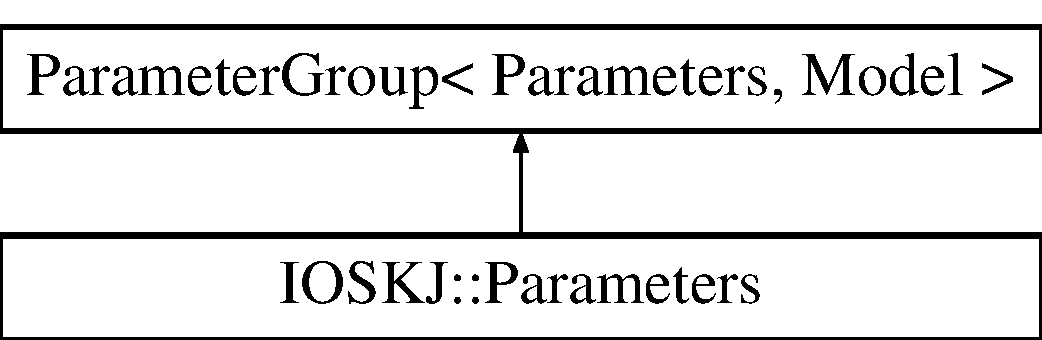
\includegraphics[height=2.000000cm]{classIOSKJ_1_1Parameters}
\end{center}
\end{figure}
\subsection*{Public Member Functions}
\begin{DoxyCompactItemize}
\item 
uint \hyperlink{classIOSKJ_1_1Parameters_a92333cb837e763080f8ebf1ea569f5fe}{first} (void) const 
\item 
\hypertarget{classIOSKJ_1_1Parameters_a7a3a67c846eec0ccff2f2cae7e918bf3}{uint {\bfseries last} (void) const }\label{classIOSKJ_1_1Parameters_a7a3a67c846eec0ccff2f2cae7e918bf3}

\item 
{\footnotesize template$<$class Binder $>$ }\\void \hyperlink{classIOSKJ_1_1Parameters_a35b3ba97ccdeb6a8d49165488d658dcd}{bind} (Binder \&binder, \hyperlink{classIOSKJ_1_1Model}{Model} \&model, uint time)
\item 
\hypertarget{classIOSKJ_1_1Parameters_aff07d5cc2d78f10a74c19a1c428beb40}{void {\bfseries read} (void)}\label{classIOSKJ_1_1Parameters_aff07d5cc2d78f10a74c19a1c428beb40}

\item 
\hypertarget{classIOSKJ_1_1Parameters_a9772edd2980c23d53def81e2bce651f3}{void {\bfseries write} (void)}\label{classIOSKJ_1_1Parameters_a9772edd2980c23d53def81e2bce651f3}

\end{DoxyCompactItemize}
\subsection*{Public Attributes}
\begin{DoxyCompactItemize}
\item 
Parameter$<$ Uniform, Log $>$ \hyperlink{classIOSKJ_1_1Parameters_a8923bdd52289ed5e29436b222121927e}{recruits\-\_\-unfished} = \{\char`\"{}recruits\-\_\-unfished\char`\"{},15,25\}
\item 
\hypertarget{classIOSKJ_1_1Parameters_aa8c53cd54a5fa2c62ac3f5043e5af640}{Parameter$<$ Uniform $>$ {\bfseries recruits\-\_\-steepness} = \{\char`\"{}recruits\-\_\-steepness\char`\"{},0.\-7,1.\-0\}}\label{classIOSKJ_1_1Parameters_aa8c53cd54a5fa2c62ac3f5043e5af640}

\item 
\hypertarget{classIOSKJ_1_1Parameters_aa83d184e0eaf4b852fe483e70ae7e0a6}{Parameter$<$ Uniform $>$ {\bfseries recruits\-\_\-sd} = \{\char`\"{}recruits\-\_\-sd\char`\"{},0.\-4,0.\-8\}}\label{classIOSKJ_1_1Parameters_aa83d184e0eaf4b852fe483e70ae7e0a6}

\item 
Parameter$<$ Truncated$<$ Normal $>$\\*
, Log $>$ \hyperlink{classIOSKJ_1_1Parameters_a083c2112ccc41ef2b0788feb08bee150}{recruits\-\_\-deviation} = \{\char`\"{}recruits\-\_\-deviation\char`\"{},0,0.\-6,-\/3,3\}
\item 
Parameter$<$ Uniform $>$ \hyperlink{classIOSKJ_1_1Parameters_a28bbbb27c4d4ae15fa93469b93553fd6}{spawning\-\_\-0} = \{\char`\"{}spawning\-\_\-0\char`\"{},0.\-7,1\}
\item 
\hypertarget{classIOSKJ_1_1Parameters_aeef621e20370efdd7f5233835109a656}{Parameter$<$ Uniform $>$ {\bfseries spawning\-\_\-1} = \{\char`\"{}spawning\-\_\-1\char`\"{},0.\-3,0.\-7\}}\label{classIOSKJ_1_1Parameters_aeef621e20370efdd7f5233835109a656}

\item 
\hypertarget{classIOSKJ_1_1Parameters_a19e1a0c82f66a22b835f960f9275b3e5}{Parameter$<$ Uniform $>$ {\bfseries spawning\-\_\-2} = \{\char`\"{}spawning\-\_\-2\char`\"{},0.\-7,1\}}\label{classIOSKJ_1_1Parameters_a19e1a0c82f66a22b835f960f9275b3e5}

\item 
\hypertarget{classIOSKJ_1_1Parameters_a8a42034667ab64402a2506525865d106}{Parameter$<$ Uniform $>$ {\bfseries spawning\-\_\-3} = \{\char`\"{}spawning\-\_\-3\char`\"{},0.\-3,0.\-7\}}\label{classIOSKJ_1_1Parameters_a8a42034667ab64402a2506525865d106}

\item 
Parameter$<$ Uniform $>$ \hyperlink{classIOSKJ_1_1Parameters_a9631eb719ef2cb669a3214d3377be1d8}{recruits\-\_\-regions} = \{\char`\"{}recruits\-\_\-regions\char`\"{},0.\-1,0.\-9\}
\item 
Parameter$<$ Uniform $>$ \hyperlink{classIOSKJ_1_1Parameters_acb9ab0f89f7ceec2e8301862f0f594ec}{recruits\-\_\-lengths\-\_\-mean} = \{\char`\"{}recruits\-\_\-lengths\-\_\-mean\char`\"{},1,10\}
\item 
\hypertarget{classIOSKJ_1_1Parameters_a6004f0a5f55c0854ca825e14d3c8f051}{Parameter$<$ Uniform $>$ {\bfseries recruits\-\_\-lengths\-\_\-cv} = \{\char`\"{}recruits\-\_\-lengths\-\_\-cv\char`\"{},0.\-1,0.\-2\}}\label{classIOSKJ_1_1Parameters_a6004f0a5f55c0854ca825e14d3c8f051}

\item 
Parameter$<$ Uniform $>$ \hyperlink{classIOSKJ_1_1Parameters_a522571c48a9b3e5c82315da4f3498865}{weight\-\_\-a} = \{\char`\"{}weight\-\_\-a\char`\"{},5.\-32e-\/6,5.\-32001e-\/6\}
\item 
\hypertarget{classIOSKJ_1_1Parameters_ad0ce26cf117948f8dfe48339523dae48}{Parameter$<$ Uniform $>$ {\bfseries weight\-\_\-b} = \{\char`\"{}weight\-\_\-b\char`\"{},3.\-35,3.\-35001\}}\label{classIOSKJ_1_1Parameters_ad0ce26cf117948f8dfe48339523dae48}

\item 
Parameter$<$ Uniform $>$ \hyperlink{classIOSKJ_1_1Parameters_a29585748679da64389d2ba756da72c99}{maturity\-\_\-inflection} = \{\char`\"{}maturity\-\_\-inflection\char`\"{},40,45\}
\item 
\hypertarget{classIOSKJ_1_1Parameters_a9c3a9534cfe6168f3e8acafe118e3945}{Parameter$<$ Uniform $>$ {\bfseries maturity\-\_\-steepness} = \{\char`\"{}maturity\-\_\-steepness\char`\"{},4,6\}}\label{classIOSKJ_1_1Parameters_a9c3a9534cfe6168f3e8acafe118e3945}

\item 
Parameter$<$ Uniform $>$ \hyperlink{classIOSKJ_1_1Parameters_a3f7804d8ec305804a0a697abcb1b0042}{mortality} = \{\char`\"{}mortality\char`\"{},0.\-5,0.\-9\}
\item 
\hypertarget{classIOSKJ_1_1Parameters_a17b1018f35ffc5618c31955668c5c46c}{Parameter$<$ Fixed $>$ {\bfseries mortality\-\_\-weight\-\_\-exponent} = \{\char`\"{}mortality\-\_\-weight\-\_\-exponent\char`\"{},-\/0.\-29\}}\label{classIOSKJ_1_1Parameters_a17b1018f35ffc5618c31955668c5c46c}

\item 
\hypertarget{classIOSKJ_1_1Parameters_a538b748c58649f18afc76da1548f236f}{Parameter$<$ Fixed $>$ {\bfseries mortality\-\_\-max} = \{\char`\"{}mortality\-\_\-max\char`\"{},-\/std\-::log(0.\-01)\}}\label{classIOSKJ_1_1Parameters_a538b748c58649f18afc76da1548f236f}

\item 
Parameter$<$ Fixed $>$ \hyperlink{classIOSKJ_1_1Parameters_a21e9e39539dc623a6d4a179f52c243d6}{growth\-\_\-rate} = \{\char`\"{}growth\-\_\-rate\char`\"{},0.\-3\}
\item 
\hypertarget{classIOSKJ_1_1Parameters_a8bd1dc029fb4e47b43bf2608e2879a00}{Parameter$<$ Fixed $>$ {\bfseries growth\-\_\-assymptote} = \{\char`\"{}growth\-\_\-assymptote\char`\"{},75\}}\label{classIOSKJ_1_1Parameters_a8bd1dc029fb4e47b43bf2608e2879a00}

\item 
\hypertarget{classIOSKJ_1_1Parameters_a43d6ae91f8b5c649e81983689e007ab7}{Parameter$<$ Fixed $>$ {\bfseries growth\-\_\-sd} = \{\char`\"{}growth\-\_\-sd\char`\"{},1\}}\label{classIOSKJ_1_1Parameters_a43d6ae91f8b5c649e81983689e007ab7}

\item 
\hypertarget{classIOSKJ_1_1Parameters_abec19913eca67fc0d0ad6fe164ef2043}{Parameter$<$ Fixed $>$ {\bfseries growth\-\_\-cv} = \{\char`\"{}growth\-\_\-cv\char`\"{},0.\-2\}}\label{classIOSKJ_1_1Parameters_abec19913eca67fc0d0ad6fe164ef2043}

\item 
Parameter$<$ Uniform $>$ \hyperlink{classIOSKJ_1_1Parameters_ab82e4c48509a372fde55b33e0a5823e6}{movement\-\_\-stay} = \{\char`\"{}movement\-\_\-stay\char`\"{},0.\-6,1.\-0\}
\item 
\hypertarget{classIOSKJ_1_1Parameters_a8eafe79341f14e09581c46cd58e527c2}{Parameter$<$ Uniform $>$ {\bfseries movement\-\_\-w\-\_\-m} = \{\char`\"{}movement\-\_\-w\-\_\-m\char`\"{},0.\-0,0.\-4\}}\label{classIOSKJ_1_1Parameters_a8eafe79341f14e09581c46cd58e527c2}

\item 
\hypertarget{classIOSKJ_1_1Parameters_a411d4a6310c09e9d07c6d02066c0f1ee}{Parameter$<$ Uniform $>$ {\bfseries movement\-\_\-m\-\_\-e} = \{\char`\"{}movement\-\_\-m\-\_\-e\char`\"{},0.\-0,0.\-4\}}\label{classIOSKJ_1_1Parameters_a411d4a6310c09e9d07c6d02066c0f1ee}

\item 
\hypertarget{classIOSKJ_1_1Parameters_abc04596c2285f5cdbac3dd1a7be55dcd}{Parameter$<$ Uniform $>$ {\bfseries movement\-\_\-w\-\_\-e} = \{\char`\"{}movement\-\_\-w\-\_\-e\char`\"{},0.\-0,0.\-2\}}\label{classIOSKJ_1_1Parameters_abc04596c2285f5cdbac3dd1a7be55dcd}

\item 
Grid$<$ Parameter$<$ Uniform $>$\\*
, Selectivity\-Knot $>$ \hyperlink{classIOSKJ_1_1Parameters_a5a522175284238012b5c49d7bd33a85a}{selectivity}
\item 
Grid$<$ Parameter$<$ Fixed $>$, \hyperlink{classIOSKJ_1_1Year}{Year}, \\*
Quarter, Region, Method $>$ \hyperlink{classIOSKJ_1_1Parameters_abc031aa9ac8ebeb935c3215d9bae0b55}{catches}
\end{DoxyCompactItemize}


\subsection{Detailed Description}
Class for defining model parameters, their priors, transformations etc. See the {\ttfamily \hyperlink{classIOSKJ_1_1Parameters_a35b3ba97ccdeb6a8d49165488d658dcd}{bind()}} method which \char`\"{}binds\char`\"{} parameters defined here to model variables. 

\subsection{Member Function Documentation}
\hypertarget{classIOSKJ_1_1Parameters_a35b3ba97ccdeb6a8d49165488d658dcd}{\index{I\-O\-S\-K\-J\-::\-Parameters@{I\-O\-S\-K\-J\-::\-Parameters}!bind@{bind}}
\index{bind@{bind}!IOSKJ::Parameters@{I\-O\-S\-K\-J\-::\-Parameters}}
\subsubsection[{bind}]{\setlength{\rightskip}{0pt plus 5cm}template$<$class Binder $>$ void I\-O\-S\-K\-J\-::\-Parameters\-::bind (
\begin{DoxyParamCaption}
\item[{Binder \&}]{binder, }
\item[{{\bf Model} \&}]{model, }
\item[{uint}]{time}
\end{DoxyParamCaption}
)\hspace{0.3cm}{\ttfamily [inline]}}}\label{classIOSKJ_1_1Parameters_a35b3ba97ccdeb6a8d49165488d658dcd}
Bind parameters to model variables \hypertarget{classIOSKJ_1_1Parameters_a92333cb837e763080f8ebf1ea569f5fe}{\index{I\-O\-S\-K\-J\-::\-Parameters@{I\-O\-S\-K\-J\-::\-Parameters}!first@{first}}
\index{first@{first}!IOSKJ::Parameters@{I\-O\-S\-K\-J\-::\-Parameters}}
\subsubsection[{first}]{\setlength{\rightskip}{0pt plus 5cm}uint I\-O\-S\-K\-J\-::\-Parameters\-::first (
\begin{DoxyParamCaption}
\item[{void}]{}
\end{DoxyParamCaption}
) const\hspace{0.3cm}{\ttfamily [inline]}}}\label{classIOSKJ_1_1Parameters_a92333cb837e763080f8ebf1ea569f5fe}
Define first and last time for parameter binding The {\ttfamily bind} method is called over this range to generate a parameter set 

\subsection{Member Data Documentation}
\hypertarget{classIOSKJ_1_1Parameters_abc031aa9ac8ebeb935c3215d9bae0b55}{\index{I\-O\-S\-K\-J\-::\-Parameters@{I\-O\-S\-K\-J\-::\-Parameters}!catches@{catches}}
\index{catches@{catches}!IOSKJ::Parameters@{I\-O\-S\-K\-J\-::\-Parameters}}
\subsubsection[{catches}]{\setlength{\rightskip}{0pt plus 5cm}Grid$<$ Parameter$<$Fixed$>$, {\bf Year},Quarter,Region,Method $>$ I\-O\-S\-K\-J\-::\-Parameters\-::catches}}\label{classIOSKJ_1_1Parameters_abc031aa9ac8ebeb935c3215d9bae0b55}
Catches by year, quarter, region and method \hypertarget{classIOSKJ_1_1Parameters_a21e9e39539dc623a6d4a179f52c243d6}{\index{I\-O\-S\-K\-J\-::\-Parameters@{I\-O\-S\-K\-J\-::\-Parameters}!growth\-\_\-rate@{growth\-\_\-rate}}
\index{growth\-\_\-rate@{growth\-\_\-rate}!IOSKJ::Parameters@{I\-O\-S\-K\-J\-::\-Parameters}}
\subsubsection[{growth\-\_\-rate}]{\setlength{\rightskip}{0pt plus 5cm}Parameter$<$Fixed$>$ I\-O\-S\-K\-J\-::\-Parameters\-::growth\-\_\-rate = \{\char`\"{}growth\-\_\-rate\char`\"{},0.\-3\}}}\label{classIOSKJ_1_1Parameters_a21e9e39539dc623a6d4a179f52c243d6}
Growth rate parameters \hypertarget{classIOSKJ_1_1Parameters_a29585748679da64389d2ba756da72c99}{\index{I\-O\-S\-K\-J\-::\-Parameters@{I\-O\-S\-K\-J\-::\-Parameters}!maturity\-\_\-inflection@{maturity\-\_\-inflection}}
\index{maturity\-\_\-inflection@{maturity\-\_\-inflection}!IOSKJ::Parameters@{I\-O\-S\-K\-J\-::\-Parameters}}
\subsubsection[{maturity\-\_\-inflection}]{\setlength{\rightskip}{0pt plus 5cm}Parameter$<$Uniform$>$ I\-O\-S\-K\-J\-::\-Parameters\-::maturity\-\_\-inflection = \{\char`\"{}maturity\-\_\-inflection\char`\"{},40,45\}}}\label{classIOSKJ_1_1Parameters_a29585748679da64389d2ba756da72c99}
Maturity parameters \hypertarget{classIOSKJ_1_1Parameters_a3f7804d8ec305804a0a697abcb1b0042}{\index{I\-O\-S\-K\-J\-::\-Parameters@{I\-O\-S\-K\-J\-::\-Parameters}!mortality@{mortality}}
\index{mortality@{mortality}!IOSKJ::Parameters@{I\-O\-S\-K\-J\-::\-Parameters}}
\subsubsection[{mortality}]{\setlength{\rightskip}{0pt plus 5cm}Parameter$<$Uniform$>$ I\-O\-S\-K\-J\-::\-Parameters\-::mortality = \{\char`\"{}mortality\char`\"{},0.\-5,0.\-9\}}}\label{classIOSKJ_1_1Parameters_a3f7804d8ec305804a0a697abcb1b0042}
Mortality parameters \hypertarget{classIOSKJ_1_1Parameters_ab82e4c48509a372fde55b33e0a5823e6}{\index{I\-O\-S\-K\-J\-::\-Parameters@{I\-O\-S\-K\-J\-::\-Parameters}!movement\-\_\-stay@{movement\-\_\-stay}}
\index{movement\-\_\-stay@{movement\-\_\-stay}!IOSKJ::Parameters@{I\-O\-S\-K\-J\-::\-Parameters}}
\subsubsection[{movement\-\_\-stay}]{\setlength{\rightskip}{0pt plus 5cm}Parameter$<$Uniform$>$ I\-O\-S\-K\-J\-::\-Parameters\-::movement\-\_\-stay = \{\char`\"{}movement\-\_\-stay\char`\"{},0.\-6,1.\-0\}}}\label{classIOSKJ_1_1Parameters_ab82e4c48509a372fde55b33e0a5823e6}
Movements parameters

There are 9 movement parameters (3 x 3 regions) but they are parameterised into 4 priors. {\ttfamily movement\-\_\-stay} defines a prior on the proportion of fish that remain in an area \hypertarget{classIOSKJ_1_1Parameters_a083c2112ccc41ef2b0788feb08bee150}{\index{I\-O\-S\-K\-J\-::\-Parameters@{I\-O\-S\-K\-J\-::\-Parameters}!recruits\-\_\-deviation@{recruits\-\_\-deviation}}
\index{recruits\-\_\-deviation@{recruits\-\_\-deviation}!IOSKJ::Parameters@{I\-O\-S\-K\-J\-::\-Parameters}}
\subsubsection[{recruits\-\_\-deviation}]{\setlength{\rightskip}{0pt plus 5cm}Parameter$<$Truncated$<$Normal$>$,Log$>$ I\-O\-S\-K\-J\-::\-Parameters\-::recruits\-\_\-deviation = \{\char`\"{}recruits\-\_\-deviation\char`\"{},0,0.\-6,-\/3,3\}}}\label{classIOSKJ_1_1Parameters_a083c2112ccc41ef2b0788feb08bee150}
Recruitment deviations \hypertarget{classIOSKJ_1_1Parameters_acb9ab0f89f7ceec2e8301862f0f594ec}{\index{I\-O\-S\-K\-J\-::\-Parameters@{I\-O\-S\-K\-J\-::\-Parameters}!recruits\-\_\-lengths\-\_\-mean@{recruits\-\_\-lengths\-\_\-mean}}
\index{recruits\-\_\-lengths\-\_\-mean@{recruits\-\_\-lengths\-\_\-mean}!IOSKJ::Parameters@{I\-O\-S\-K\-J\-::\-Parameters}}
\subsubsection[{recruits\-\_\-lengths\-\_\-mean}]{\setlength{\rightskip}{0pt plus 5cm}Parameter$<$Uniform$>$ I\-O\-S\-K\-J\-::\-Parameters\-::recruits\-\_\-lengths\-\_\-mean = \{\char`\"{}recruits\-\_\-lengths\-\_\-mean\char`\"{},1,10\}}}\label{classIOSKJ_1_1Parameters_acb9ab0f89f7ceec2e8301862f0f594ec}
\hyperlink{classIOSKJ_1_1Parameters}{Parameters} of the distribution of the lengths of recruits \hypertarget{classIOSKJ_1_1Parameters_a9631eb719ef2cb669a3214d3377be1d8}{\index{I\-O\-S\-K\-J\-::\-Parameters@{I\-O\-S\-K\-J\-::\-Parameters}!recruits\-\_\-regions@{recruits\-\_\-regions}}
\index{recruits\-\_\-regions@{recruits\-\_\-regions}!IOSKJ::Parameters@{I\-O\-S\-K\-J\-::\-Parameters}}
\subsubsection[{recruits\-\_\-regions}]{\setlength{\rightskip}{0pt plus 5cm}Parameter$<$Uniform$>$ I\-O\-S\-K\-J\-::\-Parameters\-::recruits\-\_\-regions = \{\char`\"{}recruits\-\_\-regions\char`\"{},0.\-1,0.\-9\}}}\label{classIOSKJ_1_1Parameters_a9631eb719ef2cb669a3214d3377be1d8}
Proportion of recruits by region Prior same for all regions. These are normalised in the model initialisation so that they sum to one. \hypertarget{classIOSKJ_1_1Parameters_a8923bdd52289ed5e29436b222121927e}{\index{I\-O\-S\-K\-J\-::\-Parameters@{I\-O\-S\-K\-J\-::\-Parameters}!recruits\-\_\-unfished@{recruits\-\_\-unfished}}
\index{recruits\-\_\-unfished@{recruits\-\_\-unfished}!IOSKJ::Parameters@{I\-O\-S\-K\-J\-::\-Parameters}}
\subsubsection[{recruits\-\_\-unfished}]{\setlength{\rightskip}{0pt plus 5cm}Parameter$<$Uniform,Log$>$ I\-O\-S\-K\-J\-::\-Parameters\-::recruits\-\_\-unfished = \{\char`\"{}recruits\-\_\-unfished\char`\"{},15,25\}}}\label{classIOSKJ_1_1Parameters_a8923bdd52289ed5e29436b222121927e}
\hyperlink{classIOSKJ_1_1Parameters}{Parameters} of the stock-\/recruitment relationship \hypertarget{classIOSKJ_1_1Parameters_a5a522175284238012b5c49d7bd33a85a}{\index{I\-O\-S\-K\-J\-::\-Parameters@{I\-O\-S\-K\-J\-::\-Parameters}!selectivity@{selectivity}}
\index{selectivity@{selectivity}!IOSKJ::Parameters@{I\-O\-S\-K\-J\-::\-Parameters}}
\subsubsection[{selectivity}]{\setlength{\rightskip}{0pt plus 5cm}Grid$<$ Parameter$<$Uniform$>$, Selectivity\-Knot $>$ I\-O\-S\-K\-J\-::\-Parameters\-::selectivity}}\label{classIOSKJ_1_1Parameters_a5a522175284238012b5c49d7bd33a85a}
{\bfseries Initial value\-:}
\begin{DoxyCode}
= \{
        Parameter<Uniform>
        \{\textcolor{stringliteral}{"selectivity\_20"},0,0.3\},
        \{\textcolor{stringliteral}{"selectivity\_30"},0,0.4\},
        \{\textcolor{stringliteral}{"selectivity\_40"},0,0.6\},
        \{\textcolor{stringliteral}{"selectivity\_50"},0,1\},
        \{\textcolor{stringliteral}{"selectivity\_60"},0,1\},
        \{\textcolor{stringliteral}{"selectivity\_70"},0,1\},
        \{\textcolor{stringliteral}{"selectivity\_80"},0,1\}
    \}
\end{DoxyCode}
Selectivity parameters

These are likely to be well determined from the data and so a U(0,1) prior is used for all \hypertarget{classIOSKJ_1_1Parameters_a28bbbb27c4d4ae15fa93469b93553fd6}{\index{I\-O\-S\-K\-J\-::\-Parameters@{I\-O\-S\-K\-J\-::\-Parameters}!spawning\-\_\-0@{spawning\-\_\-0}}
\index{spawning\-\_\-0@{spawning\-\_\-0}!IOSKJ::Parameters@{I\-O\-S\-K\-J\-::\-Parameters}}
\subsubsection[{spawning\-\_\-0}]{\setlength{\rightskip}{0pt plus 5cm}Parameter$<$Uniform$>$ I\-O\-S\-K\-J\-::\-Parameters\-::spawning\-\_\-0 = \{\char`\"{}spawning\-\_\-0\char`\"{},0.\-7,1\}}}\label{classIOSKJ_1_1Parameters_a28bbbb27c4d4ae15fa93469b93553fd6}
Proportion of mature fish spawning by quarter \hypertarget{classIOSKJ_1_1Parameters_a522571c48a9b3e5c82315da4f3498865}{\index{I\-O\-S\-K\-J\-::\-Parameters@{I\-O\-S\-K\-J\-::\-Parameters}!weight\-\_\-a@{weight\-\_\-a}}
\index{weight\-\_\-a@{weight\-\_\-a}!IOSKJ::Parameters@{I\-O\-S\-K\-J\-::\-Parameters}}
\subsubsection[{weight\-\_\-a}]{\setlength{\rightskip}{0pt plus 5cm}Parameter$<$Uniform$>$ I\-O\-S\-K\-J\-::\-Parameters\-::weight\-\_\-a = \{\char`\"{}weight\-\_\-a\char`\"{},5.\-32e-\/6,5.\-32001e-\/6\}}}\label{classIOSKJ_1_1Parameters_a522571c48a9b3e5c82315da4f3498865}
Length-\/weight parameters 

The documentation for this class was generated from the following file\-:\begin{DoxyCompactItemize}
\item 
parameters.\-hpp\end{DoxyCompactItemize}

\hypertarget{structIOSKJ_1_1Tracker}{\section{I\-O\-S\-K\-J\-:\-:Tracker Struct Reference}
\label{structIOSKJ_1_1Tracker}\index{I\-O\-S\-K\-J\-::\-Tracker@{I\-O\-S\-K\-J\-::\-Tracker}}
}


{\ttfamily \#include $<$tracker.\-hpp$>$}

\subsection*{Public Member Functions}
\begin{DoxyCompactItemize}
\item 
\hypertarget{structIOSKJ_1_1Tracker_afa56ecd201a5cf1c7b5830098b3dc6ef}{{\bfseries Tracker} (std\-::string path)}\label{structIOSKJ_1_1Tracker_afa56ecd201a5cf1c7b5830098b3dc6ef}

\item 
\hypertarget{structIOSKJ_1_1Tracker_a01092eb7b77b78fce12d15a13ebd5e51}{void {\bfseries get} (const \hyperlink{classIOSKJ_1_1Model}{Model} \&model, uint time)}\label{structIOSKJ_1_1Tracker_a01092eb7b77b78fce12d15a13ebd5e51}

\end{DoxyCompactItemize}
\subsection*{Public Attributes}
\begin{DoxyCompactItemize}
\item 
\hypertarget{structIOSKJ_1_1Tracker_ad2bef8b4314ba5399e42e251ebecf129}{std\-::ofstream {\bfseries file}}\label{structIOSKJ_1_1Tracker_ad2bef8b4314ba5399e42e251ebecf129}

\end{DoxyCompactItemize}


\subsection{Detailed Description}
Tracking of various model variables during simulation. Mainly used in testing. 

The documentation for this struct was generated from the following file\-:\begin{DoxyCompactItemize}
\item 
tracker.\-hpp\end{DoxyCompactItemize}

\hypertarget{classIOSKJ_1_1Year}{\section{I\-O\-S\-K\-J\-:\-:Year Class Reference}
\label{classIOSKJ_1_1Year}\index{I\-O\-S\-K\-J\-::\-Year@{I\-O\-S\-K\-J\-::\-Year}}
}
Inheritance diagram for I\-O\-S\-K\-J\-:\-:Year\-:\begin{figure}[H]
\begin{center}
\leavevmode
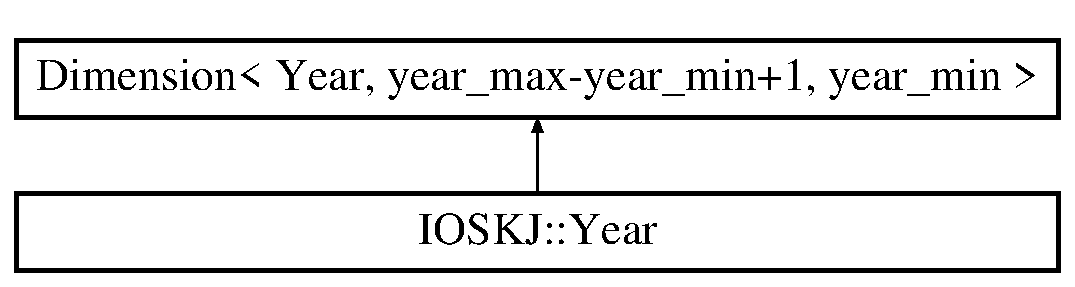
\includegraphics[height=2.000000cm]{classIOSKJ_1_1Year}
\end{center}
\end{figure}
\subsection*{Static Public Member Functions}
\begin{DoxyCompactItemize}
\item 
\hypertarget{classIOSKJ_1_1Year_a6e310c45eb605b1464b2bc47873afca0}{static const char $\ast$ {\bfseries name} (void)}\label{classIOSKJ_1_1Year_a6e310c45eb605b1464b2bc47873afca0}

\end{DoxyCompactItemize}


The documentation for this class was generated from the following file\-:\begin{DoxyCompactItemize}
\item 
dimensions.\-hpp\end{DoxyCompactItemize}

%--- End generated contents ---

% Index
\newpage
\phantomsection
\addcontentsline{toc}{part}{Index}
\printindex

\end{document}
